\documentclass[12pt]{article}
\usepackage[utf8]{inputenc}
\usepackage{graphicx}
\usepackage{xcolor}
\usepackage[a4paper,width=150mm,top=25mm,bottom=25mm]{geometry}

\title{
{\includegraphics[width=300px, height=200px]{OT.png}}
\\
{Travel Agency Software Proposal }
}
\date{}
\begin{document}

\maketitle
\newpage

\begin{center}
\section*{\textcolor [HTML]{32CD32} {Odyssey Travels} : Your Passport to Adventure }
\vspace{10px}
\end{center}
\subsection*{\fontsize{14}{0}\selectfont Project Description }
 We  are presenting a proposal for the development of a robust website for a travel agency, offering users the ability to explore diverse travel packages, customize their itineraries, book flights, and make payments seamlessly. Our goal is to create a user-centric platform that simplifies the travel booking process while ensuring security and convenience for customers.

\subsection*{\fontsize{14}{0}\selectfont Project Features }
\begin{itemize}
    \item \textbf{Package Exploration:} Users can browse through a diverse range of travel packages, including destination highlights, activities, and accommodation options.
    
    \item \textbf{Customization Options:} The website will allow users to tailor their travel itineraries by selecting specific destinations, activities, and travel dates.
    
    \item \textbf{Flight Booking:} Integration with a reliable flight booking system will enable users to search for and book flights directly through the website.
    
    \item \textbf{User Profiles:} Users can create accounts to manage their bookings, preferences, and past travel history.
    
    \item \textbf{Payment Gateway:} Secure payment processing for booking confirmations, including support for multiple currencies and payment methods.
    
    \item \textbf{Reviews and Ratings:} Users can provide feedback and ratings for destinations, accommodations, and overall travel experiences.
    
    \item \textbf{Responsive Design:} Ensuring optimal performance and accessibility across various devices, including desktops, tablets, and smartphones.
\end{itemize}


\subsection*{Project Plan }

{
\subsection*{\fontsize{13}{0}\selectfont Phase 1: Planning and Preparation}
}

\begin{itemize}
    \item Duration: 1 month
    \item Project Initiation
        \begin{itemize}
            \item Define project objectives, scope, and success criteria.
            \item Identify key stakeholders and establish communication channels.
        \end{itemize}
    \item Requirement Gathering
        \begin{itemize}
            \item Conduct interviews and workshops with internal stakeholders to gather functional and technical requirements.
            \item Prioritize features and define user stories.
        \end{itemize}
    \item Resource Allocation
        \begin{itemize}
            \item Allocate human and technical resources required for software development.
            \item Set up development environment and infrastructure.
        \end{itemize}
\end{itemize}

\subsection*{\fontsize{13}{0}\selectfont Phase 2: Design and Development}

\begin{itemize}
    \item Duration: 4 months
    \item UI/UX Design
        \begin{itemize}
            \item Develop wireframes and mockups for the user interface.
            \item Gather feedback from stakeholders and iterate on design.
        \end{itemize}
    \item Database Design
        \begin{itemize}
            \item Design the database schema to support the required functionality.
            \item Determine data storage and retrieval mechanisms.
        \end{itemize}
    \item Backend Development
        \begin{itemize}
            \item Develop server-side logic and APIs to support client interactions.
            \item Implement business logic for booking management, payment processing, and itinerary generation.
        \end{itemize}
    \item Frontend Development
        \begin{itemize}
            \item Develop client-side interfaces for the customer portal and administrative dashboard.
            \item Implement responsive design and ensure cross-browser compatibility.
        \end{itemize}
    \item Integration
        \begin{itemize}
            \item Integrate third-party services, such as payment gateways and CRM systems, as needed.
            \item Conduct thorough testing to ensure seamless integration.
        \end{itemize}
\end{itemize}

\subsection*{\fontsize{13}{0}\selectfont Phase 3: Testing and Quality Assurance}

\begin{itemize}
    \item Duration: 1 month
    \item Unit Testing
        \begin{itemize}
            \item Test individual components and functions to identify bugs and errors.
            \item Use automated testing tools for regression testing.
        \end{itemize}
    \item Integration Testing
        \begin{itemize}
            \item Test the interaction between different modules and subsystems.
            \item Verify data flow and system behaviour under various scenarios.
        \end{itemize}
    \item User Acceptance Testing (UAT)
        \begin{itemize}
            \item Invite stakeholders and end-users to participate in UAT.
            \item Gather feedback and address any usability issues or discrepancies.
        \end{itemize}
\end{itemize}

\subsection*{\fontsize{13}{0}\selectfont Phase 4: Deployment and Launch}

\begin{itemize}
    \item Duration: 1 month
    \item Deployment
        \begin{itemize}
            \item Deploy the software to production servers or cloud infrastructure.
            \item Configure monitoring and logging systems for performance tracking.
        \end{itemize}
    \item Training
        \begin{itemize}
            \item Conduct training sessions for internal users on how to use the software.
            \item Provide documentation and support materials for reference.
        \end{itemize}
    \item Soft Launch
        \begin{itemize}
            \item Roll out the software to a limited audience for initial feedback and testing.
            \item Monitor system performance and address any issues in real time.
        \end{itemize}
\end{itemize}

\subsection*{\fontsize{13}{0}\selectfont Phase 5: Post-Launch Support and Maintenance}

\begin{itemize}
    \item Duration: Ongoing
    \item Bug Fixing and Optimization
        \begin{itemize}
            \item Continuously monitor and address bugs reported by users.
            \item Optimize system performance and scalability as needed.
        \end{itemize}
    \item Feature Enhancements
        \begin{itemize}
            \item Gather feedback from users and stakeholders to prioritize feature enhancements.
            \item Plan and implement updates and new features in iterative cycles.
        \end{itemize}
    \item Technical Support
        \begin{itemize}
            \item Provide ongoing technical support to users through various channels, including email, chat, and phone.
            \item Respond to inquiries and troubleshoot issues on time.
        \end{itemize}
\end{itemize}
 
\subsection * {Background / Motivation}
The travel industry has undergone significant transformations in recent years, driven by technological advancements and changing consumer preferences. In this dynamic landscape, travelers seek convenient and personalized solutions that simplify the process of planning and booking their trips. As such, there is a growing demand for online platforms that offer comprehensive travel services, from exploring destination options to booking flights and accommodations.\newline Traditional methods of travel planning often involve extensive research across multiple websites, making it time-consuming and cumbersome for travelers to finalize their itineraries. Moreover, the lack of customization options and limited access to real-time information can hinder the overall travel experience.\newline In response to these challenges, there is a clear need for a centralized platform that streamlines the entire travel booking process while providing users with greater flexibility and control over their travel plans. By integrating features such as package exploration, customization options, flight booking, and secure payment gateways, we aim to address these pain points and elevate the travel booking experience for customers.\newline Furthermore, the COVID-19 pandemic has reshaped the way people approach travel, with safety and flexibility becoming paramount concerns. A robust online platform that offers transparent information, flexible booking policies, and seamless payment options will not only meet the evolving needs of travelers but also instill confidence and trust in the travel agency's services.\newline In summary, the motivation behind this project stems from the desire to revolutionize the way travelers plan and book their trips. By leveraging technology to create a user-centric travel agency website, we aim to enhance convenience, accessibility, and satisfaction for customers, ultimately establishing the travel agency as a leading player in the competitive travel industry.
\subsection * { Budget Analysis : Odyssey Travels \& Tours Project }
\begin{enumerate}
    \item \textbf{Development Costs:}
    \begin{itemize}
        \item Software Development Team Salaries: \$200,000
        \item Infrastructure Setup (Servers, Cloud Services): \$50,000
        \item Software Tools and Licenses: \$20,000
    \end{itemize}
    
    \item \textbf{Design Expenses:}
    \begin{itemize}
        \item UI/UX Design Services: \$30,000
        \item Graphic Design and Branding: \$15,000
    \end{itemize}
    
    \item \textbf{Testing and Quality Assurance:}
    \begin{itemize}
        \item Testing Tools and Software: \$10,000
        \item QA Team Salaries: \$50,000
    \end{itemize}
    
    \item \textbf{Deployment and Training:}
    \begin{itemize}
        \item Deployment Costs (Hosting, Domain): \$10,000
        \item User Training and Documentation: \$15,000
    \end{itemize}
    
    \item \textbf{Marketing and Promotion:}
    \begin{itemize}
        \item Website Development and Marketing Collateral: \$25,000
        \item Digital Marketing Campaigns: \$50,000
    \end{itemize}
    
    \item \textbf{Contingency Fund (10\% of Total Budget):} \$45,000
\end{enumerate}

\noindent\textbf{Total Estimated Budget:} \$520,000

\noindent\textbf{Note:} The budget analysis provides a rough estimate of the costs involved in developing and launching the WorldWander project. Actual expenses may vary depending on factors such as team size, project scope, and specific requirements. Adjustments can be made to the budget breakdown based on detailed project planning and resource allocation.


\section * {UML Diagram For Travel Agency Software}
\title{
{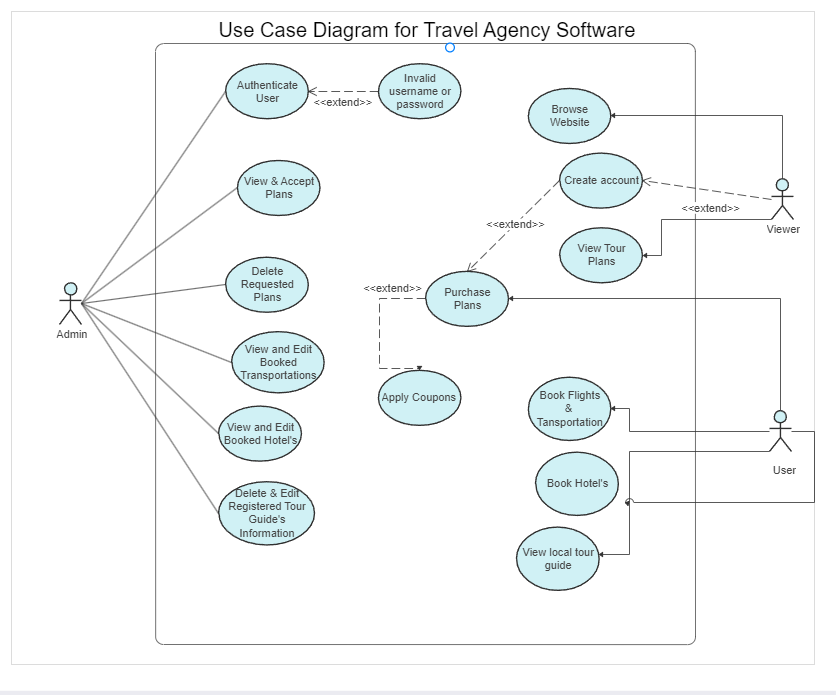
\includegraphics[width=450px, height=300px]{uml.png}}

\section * {Software Requirements : }
\subsection*{Technologies will be used :}
\begin{itemize}
    \item Next.js
    \item Tailwind CSS
    \item Ant Design
    \item Deysi UI
    \item Firebase (for authentication, database, and hosting)
    \item Toastify (for notifications)
    \item Node.js
    \item Express.js
    \item MySQL (as the relational database)
\end{itemize}
  
\subsection*{Additional Tools:}
\begin{itemize}
    \item Visual Studio Code (for development)
    \item Git and GitHub (for version control)
    \item Figma (for UI/UX design and prototyping)
    \item Postman (for API testing)
    \item Swagger (for API documentation)
\end{itemize}

\subsection*{Proposed Additional Features:}
\begin{itemize}
    \item User Authentication
    \item Trip Management
    \item Booking Management
    \item Payment Integration
    \item User Dashboard
    \item Admin Panel
    \item Search and Filter
    \item Responsive Design
    \item Notifications
    \item Performance Optimization
    \item API Documentation
    \item Security Measures
    \item Testing
    \item Deployment
\end{itemize}

\subsection*{Project Timeline:}
\begin{itemize}
    \item Week 1-2: Requirement gathering and planning.
    \item Week 3-4: Setting up project structure and authentication.
    \item Week 5-6: Developing trip management functionalities.
    \item Week 7-8: Implementing booking management and payment integration.
    \item Week 9-10: Testing, debugging, and optimization.
    \item Week 11-12: Final testing, deployment, and documentation.
\end{itemize}

\section * {Conclusion}
In the realm of travel, where dreams intertwine with reality, the Odyssey Travels and Tours project proposal stands as a testament to innovation and excellence. Through meticulous planning, thoughtful design, and unwavering dedication, we have outlined a vision for a groundbreaking online platform that redefines the travel booking experience. The journey through the intricacies of development, guided by the principles of agility and collaboration, we remain steadfast in our commitment to realizing this vision. With each line of code and every design element, we strive to create a digital haven where exploration knows no bounds.The Odyssey Travels and Tours project represents more than just a website; it embodies the aspirations of travelers worldwide, seeking adventure, discovery, and moments that transcend the ordinary. With features such as package exploration, customizable itineraries, seamless flight booking, and secure payment gateways, we aim to elevate the travel experience to new heights.\newline As we embark on this odyssey together, we extend our gratitude to all stakeholders for their trust and collaboration. With your continued support, we are confident that the Odyssey Travels and Tours website will not only meet but exceed expectations, becoming a beacon of inspiration for travelers far and wide.Let us embark on this journey with excitement and determination, knowing that the Odyssey awaits, ready to unveil a world of possibilities. Together, let us redefine the future of travel.

\end{document}